% !TeX encoding = UTF-8
% CABECERA
% BEGIN_FOLD
%%%%%%%%%%%%%%
% Fichero: uclmTFGesi.tex
% Autor: Jesús Salido Tercero (https://www.esi.uclm.es/www/jsalido)
% Fecha (creación): Febrero 2010 
% Rev. : Febrero 2020
% Descripción: Plantilla para memoria de TFG 
% (Escuela Sup. de Informática, UCLM). Creada para el curso 
% “LaTeX esencial para preparación de TFG, Tesis y otros documentos 
% académicos” (Esc. Sup. Informática-UCLM)
%
%### Compilación 
%
% Esta plantilla ha sido preparada para compilarse con `pdflatex`, `biblatex` 
% (bibliografía con `biber`) y `makeindex` (sólo si se incluye índice 
% temático).
%
% Para su compilación se aconseja utilizar `latexmk` (requiere para su 
% ejecución de un intérprete [`Perl`]([Win] http://strawberryperl.com/)):
%
%> \$> latexmk -pdf -silent -synctex=1  
%
% Para la automatización del trabajo con esta plantilla es recomendable el 
% empleo de IDE dedicados como [TeXstudio](https://www.texstudio.org/).
%
% Una versión revisada de esta plantilla está disponible en overleaf.
% Puede crearse un proyecto propio para escribir un TFG directamente en 
% overleaf, o bien descargarla como un archivo .zip para su utilización en 
% modo local.
%
% Si deseas acceder a la versión de desarrollo puedes encontrarla en GitHub:
%	https://github.com/JesusSalido/TFG_ESI_UCLM
%%%%%%%%%%%%%%
% END_FOLD


% -------------------------
%
% PREÁMBULO
% BEGIN_FOLD
% -------------------------
\documentclass[ 		% Clase del documento
	11pt,				% Tamaño de letra
	a4paper,			% Tamaño de papel
	twoside,			% Impresión a doble cara
	openright,			% La apertura de cap. a la dcha.
%	draft       		% Versión borrador (sin figuras)
	final       		% Versión final
]{book}

%--- Codificación de entrada (mejora respecto a inputenc)
\usepackage[utf8]{inputenx} 
\usepackage[
    english,     % Se emplea porque el resumen siempre en inglés
    spanish,     % Se emplea para resumen en español
    es-tabla,    % Si idioma pral. español
    es-noindentfirst
]{babel} % Internacionalización


%--- Geometría de las páginas del documento
\usepackage[			% Márgenes del documento
	top=2.5cm,			% Margen superior
	bottom=2.5cm,		% Margen inferior
	inner=3.5cm,		% Margen al interior
	outer=2cm			% Margen al exterior
]{geometry}

%--- Tipografía
\usepackage{amsmath,amssymb,amsfonts} % Para ecs.

%--- Si no se emplea ningún paquete de tipografía se empleará Computern Modern.
%--- Tipografía 
%--- (Opción: Latin Modern)
%\usepackage{lmodern} % Latin Modern. Empleada cuando se desea una tipografía genuina de LaTeX sucesora de Computer Modern.
%--- (Opción: Libertine)
\usepackage[tt=false]{libertine} % Libertine con Old-Style Figures [osf]
\usepackage[libertine]{newtxmath} % Times
%--- (Opción: Palatino)
%\usepackage{newpxtext} % Palatino: La opción osf proporciona números en old style.
%\usepackage{newpxmath}	% Palatino
%--- (Opción: Fourier)
%\usepackage{fourier} % Utopía
%---

%--- (Opción excepcional)
% EDITAR: Si es preciso cambio de tipo de familia de tipografía por defecto a Sans-Serif
% Aunque es una opción extraña es la preferida en algunos centros docentes (ADE-UCLM).
% Con esta elección es más conveniente una tipografía tipo Helvética/Arial (no Libertine)
%\usepackage{helvet}
%\renewcommand{\familydefault}{\sfdefault}
%---

\usepackage{textcomp,marvosym,pifont} % OPT.: Generación de símbolos 
%especiales
\usepackage{ccicons} % OPT.: Iconos de licencia Creative Commons
\usepackage[T1]{fontenc}% Codificación de salida    

%--- Paquete con personalización local para el TFG (ESI-UCLM)
% EDITAR: Si es preciso que la memoria emplee "english" como idioma 
% principal, prefijos de género y ubicación en número de página al pie.
% Con la opción "english" el resto de opciones son irrelevantes.
% Los prefijos de género permiten un tratamiento adecuado en portadas
% automáticas.
%
% Opciones del paquete: (por defecto) Memoria en español y prefijos masculinos.
%	spanish: idioma pral. español (valor por defecto).
%   english: idioma pral. inglés.
%	autora,tutora,cotutora: indica el género de intervinientes (masculino por defecto) 	
%	pageonfooter: Número de página en el pie y centrado como ADE-UCLM (por defecto en cabeceras)
% -------------------------
% COMANDOS OPCIONALES PROPORCIONADOS:
% OP-Opcional
% RE-Recomendado
%
% Comandos de generación automática de portadas
% \portadaTFG, \portadaTFG*{ficheroPDF}: Página de portada
% \portillaTFG, \portadillaTFG*{ficheroPDF}: Página de contraportada
% \tribunalTFG, \tribunalTFG*{ficheroPDF}: Página de tribunal
% \dedicado{texto}: Dedicatoria
% \creditos{texto}{fichero gráfico de licencia}
%
% Comandos para definir variables con los datos del documento.
%
% OP-\nodivide[penalty]			: Penaliza la división de palabras. Máx. 
%								: (n=10000) sin arg.
% OP-\nowidowandorphan[penalty] : Penaliza las viudas y huérfanas. (sólo si necesario)
% OP-\nodividenotes[penalty]	: Penaliza la división de notas al pié entre págs.	(sólo si necesario)	
% OP-\savepagecnt				: Salva en un contador interno el nº de pág. actual
% OP-\contpagination			: Recupera el valor de pág. previamente salvado en el cont. interno.
% OP-\tecla{texto}				: Genera un borde de tecla en torno al 
%texto		
% -------------------------
%\usepackage{uclmTFGesi}
\usepackage[tutora,cotutora]{uclmTFGesi}
%\usepackage[pageonfooter]{uclmTFGesi}



%--- Bibliografía: Biblatex con biber.
% EDITAR: Si se desea cambiar los estilos de citación y ordenación de la bibliografía
\usepackage[%
	backend=biber,
	% Estilos: numeric, numeric-comp, alphabetic, authoryear, authoryear-comp
	% Otros: apa, chicago, ieee, mla-new, iso-numeric, iso-authoryear
	% Estilos tradicionales BibTeX: trad-plain, trad-unsrt, trad-alpha y trad-abbrv
%	style=apa, % Estilo APA
	style=ieee,
	% Citación: numeric, numeric-comp, numeric-verb, 
	%           authoryear, authoryear-comp,...
	%           otros aplicados con estilo gral.: ieee,apa,aml,chem-acs,iso-numeric,iso-authoryear
	citestyle=numeric-comp,
	sortcites, % Ordenación de citas múltiples cuando son numéricas
	maxbibnames=3, % Máximo número listado de autores en la bibliografía
	minbibnames=1, % Mínimo número de autores cuando se abrevia la lista de autores
	% Descomentar las opciones siguientes para bibliografía multilingüe
	autolang=other, % Requerido para opción multilingüe
	language=auto,   % Requerido para opción multilingüe
	sorting=nyt%
					% Para cambiar criterio de ordenación de las referencias.
 					% =nty (name-title-year), nyt (name-year-title), nyvt (name-year-volume-title), 
					% =anyt (alphabetic-name-year-title), anyvt (alphabetic-name-year-volume-title), 
					% =ynt (year-name-title), ydnt (yeardescendent-name-title), 
					% =none (por orden de citación, como en ETSII-UCLM).			
]{biblatex}

% Línea añadida para eliminar el idioma de la fuente bibliográfica.
\AtEveryBibitem{\clearfield{note} \clearlist{language}}

% OPT: No comentar si es necesario suprimir el sangrado de párrafos.
%\setlength{\parindent}{0pt} % Elimina sangrado de párrafos

\addbibresource{biblioTFG.bib} 	% Fichero de bibliografía.
\graphicspath{{./figs/}}% Path de búsqueda de ficheros gráficos

\usepackage{makeidx} % OPT.: Indice temático
\makeindex           % OPT.: Procesamiento de índice temático
% END_FOLD
% -------------------------
% -------------------------
% -------------------------



% DATOS del documento
% BEGIN_FOLD
% -------------------------
% -------------------------
% -------------------------
% DATOS DEL DOCUMENTO 
% Definición de variables empleadas en el documento por lo que no son
% traducidos. Cuando algún campo puede tener varias líneas aparecen dos
% campos señalados como <campo>Primera y <campo>Segunda. Si no se desea 
% emplear los campos opcionales (OPT.) estos deben comentarse.
% -------------------------
% EDITAR: Datos del documento. 
% NOTA: Los elementos opcionales pueden dejarse, eliminarse o comentarse. No se deben dejar vacíos porque provoca errores.
\tituloPrimera{Plantilla guía de TFG para la ESI-UCLM} % 1ª Línea
\tituloSegunda{Curso de {\LaTeX{}} esencial} % OPT.: Para títulos largos.
\titulo{Plantilla guía de TFG} % Título corto (mostrado en pág. de créditos)
\autor{Jesús Salido Tercero}
\email{jesus.salido@uclm.es}					
\tutor{<tutor(a) (nombre apellidos)>} % Sólo nombre, el prefijo añadido automát.
\cotutor{<co-tutor(a) (nombre apellidos)>}	% OPT.: Cotutor(a)
\instEdu{UNIVERSIDAD DE CASTILLA-LA MANCHA}

% Fichero con escudo de la institución
% Logo de la ESI que prefieras (la normativa no especifica obligatoriedad).
%\escudo{esi} 					% Logo ESI (gris uniforme)							
%\escudo{esi_black} 			% Logo ESI (negro)						
%\escudo{esi_color}				% Logo ESI (dos tintas)						
\escudo{IngInformatica_color}	% Nucleo de ferrita	(color)
%\escudo{IngInformatica_bw} 	% Nucleo de ferrita	(en escala de grises)					

\centroEdu{ESCUELA SUPERIOR DE INFORMÁTICA}
\deptoEduPrimera{<Primera línea Depto. Director>} % 1ª Línea(EN: Department of ...)
\deptoEduSegunda{<Segunda línea Depto. Director>} % OPT.: Para nombres largos.
\titulacion{GRADO EN INGENIERÍA INFORMÁTICA} % (EN: BACHELOR IN COMPUTING ENGINEERING)
\especialidad{<Tecnología Específica>} % OPT.: Especialidad - Intensificación
% (EN: Specialization in ...)
\tipoDoc{TRABAJO FIN DE GRADO} % (EN: BACHELOR DISSERTATION)

% Si las fechas se desean en inglés hay que ponerla explícita.
\fechaDef{julio, 2021} 			% Fecha de defensa
\mesDef{julio}        			% Mes de defensa
\yearDef{2021}        			% Año de defensa
\lugarDef{Ciudad Real}			% Lugar de defensa


% --- Metadatos (propiedades) para el documento PDF
\hypersetup{% OPT.
% EDITAR: Valores para el PDF.	
	pdftitle={Plantilla guía para TFG en la UCLM}, % Título
	pdfauthor={Jesús Salido (ESI-UCLM)}, % Autor
	pdfsubject={TFG},  % Tema
	pdftoolbar=true, % Muestra la toolbar de Acrobat
	pdfmenubar=true	 % Muestra la menubar de Acrobat
}
% -------------------------
% -------------------------
% -------------------------
% END_FOLD



% -------------------------
% -------------------------
% -------------------------
% -------------------------
%
% CUERPO del documento
%
% -------------------------
\begin{document}
% PORTADAS (FRONTMATTER)
% BEGIN_FOLD
\frontmatter
% Cambia la numeración de páginas a números romanos y las secciones no están 
%numeradas aunque si aparecen en el índice de contenidos.
\pagestyle{empty}  % Páginas sin cabecera ni pies

% -------------------------
% -------------------------
% -------------------------
%
% PORTADAS: 
%
% Los comandos \portadaTFG y \portadilla generan dos portadas con LaTeX 
% teniendo en cuenta los datos sobre el documento aportados en el preámbulo.
% Si se desea incluir una portada generada externamente en PDF se emplea la
% versión del comando con estrella indicando el fichero.
%
% -------------------------





%---
% EDITAR: Si es preciso incluir portada generada externamente en PDF.
\portadaTFG		% Portada pral.
%\portadaTFG*{./portadas/portadaADE} % Portada generada externamente en PDF
%\portadaTFG*{./portadas/portadaETSII_IE} % Portada generada externamente en PDF
%\portadaTFG*{./portadas/portadaETSII_TFM} % Portada generada externamente en PDF
% También en versión con estrella para indicar fichero PDF
% Comentar si no se desea incluir
%---






%---
% EDITAR: Si es preciso incluir portada generada externamente en PDF.
\portadillaTFG	% Portada interior (con tutor(a) y co-tutor(a) si existe).
% También en versión con estrella para indicar fichero PDF
% Comentar si no se desea incluir
%---





%---
% OPT.: CRÉDITOS (aunque no es obligatorio es recomendable).
% -------------------------
%
% CRÉDITOS
%
% -------------------------
% EDITAR: El autor puede elegir el tipo de licencia que desee para distribuir su TFG que puede variar con respecto a la de este documento en el que si permitimos obra derivada para que no surjan dudas sobre la reutilización del material.
% Este comando permite una gran flexibilidad y la ventaja de no depender de paquetes externos.
% Esta es una página reservada para señalar información relativa a los derechos de autor y la licencia de distribución y uso del documento. Esta página debería ser aprovechada también para informar de cualquier tipo de cesión de los derechos anteriormente citados. El autor del TFG debe tener presente que el incumplimiento de la legislación vigente en materia de protección de la propiedad intelectual es de su exclusiva responsabilidad independientemente de la cesión de derechos que este haya convenido para su obra ya que no son objeto de cesión aquellos derechos de los que no se es poseedor.

\creditos{Este documento se distribuye con licencia CC BY-NC-SA 4.0. El texto completo de la licencia puede obtenerse en \url{https://creativecommons.org/licenses/by-nc-sa/4.0/}.

La copia y distribución de esta obra está permitida en todo el mundo, sin regalías y por cualquier medio, siempre que esta nota sea preservada. Se concede permiso para copiar y distribuir traducciones de este libro desde el español original a otro idioma, siempre que la traducción sea aprobada por el autor del libro y tanto el aviso de copyright como esta nota de permiso, sean preservados en todas las copias.

% OJO: Deja esta nota de atribución al uso de la plantilla LaTeX.
Este texto ha sido preparado con la plantilla \LaTeX{} de TFG para la UCLM publicada por \href{https://www.esi.uclm.es/www/jsalido}{Jesús Salido} en GitHub\footnote{\url{https://github.com/JesusSalido/TFG_ESI_UCLM}} y Overleaf \footnote{\url{https://www.overleaf.com/latex/templates/plantilla-de-tfg-escuela-superior-de-informatica-uclm/phjgscmfqtsw}} como parte del curso \href{http://visilab.etsii.uclm.es/?page_id=1468}{\emph{<<\LaTeX{} esencial para preparación de TFG, Tesis y otros documentos académicos>>}} impartido en la Escuela Superior de Informática de la Universidad de Castilla-La Mancha.}{by-nc-sa}


% NOTA: Para citar este documento puede emplear el registro siguiente:
%@www{salidoTFG,
%  author       = {Jesús Salido},
%  title        = {Plantilla guía de TFG para la ESI-UCLM},
%  year         = {2019},
%  editor       = {GitHub},
%  organization = {Universidad de Castilla-La Mancha},
%  url          = {https://github.com/JesusSalido/TFG_ESI_UCLM},
%}


%---



%---




%---
% EDITAR: Si es preciso incluir portada generada externamente en PDF.
\tribunalTFG % Página para calificaciones del tribunal
% También en versión con estrella para indicar fichero PDF
%---





%---
% OPT.: DEDICATORIA (1 pág. máximo) comentar si no se desea incluir.
% Aunque opcional, no se debería perder la oportunidad de poder 
% dedicar el trabajo a alguien MUY especial.
% EDITAR: Dedicatoria.
\dedicado{A mis estudiantes \\ % A alguien muy especial
Por contribuir a hacer de cada día un reto ilusionante} % Como mucho dos líneas (no confundir con los agradecimientos).
%---
%
% FIN PORTADAS: 
% |
% |
% -> ----------------------


% -------------------------
%
% RESUMEN:
%
% -------------------------
%--- Ajustes del documento.
\pagestyle{plain}	% Páginas sólo con numeración inferior al pie

% -------------------------
%
% RESUMEN:
% OJO: Si es preciso cambiar manualmente orden Resumen <-> Abstract
%
% -------------------------
%--- Resumen en español
\selectlanguage{spanish} % Selección de idioma del resumen.
\cleardoublepage % Se incluye para modificar el contador de página antes de añadir bookmark
\phantomsection  % Necesario con hyperref
\addcontentsline{toc}{chapter}{Resumen} % Añade al TOC.

\begin{abstract}
% EDITAR: Resumen (máx. 1 pág.)
\begin{center}
\emph{[... versión del resumen en español ...]}
\end{center}
En una página como máximo, el resumen explicará de modo breve la problemática que trata de resolver el trabajo \emph{(el `qué')}, la metodología para  abordar su solución  \emph{(el `cómo')} y los resultados obtenidos. En los trabajos cuyo idioma principal sea el inglés, el orden de \textsf{Resumen} y \textsf{Abstract} se invertirá.
\end{abstract}
%---



%--- Resumen en inglés
% Abstract
\selectlanguage{english} % Selección de idioma del resumen.
\cleardoublepage
\phantomsection % Necesario con hyperref
\addcontentsline{toc}{chapter}{Abstract} % Añade al TOC.

\begin{abstract}
% EDITAR: Abstract (máx. 1 pág.)

\begin{center}
\emph{[... english version of the abstract ...]}
\end{center}
English version for the abstract.	
\end{abstract}
%---

%--- Ajuste del idioma para el resto del documento.
\ifspanish
	\selectlanguage{spanish}% Emplea idioma español
\else
	\selectlanguage{english}% Emplea idioma inglés
\fi

%---


% -------------------------
%
% AGRADECIMIENTOS (recomendable máx. 1 pág.)
%
% -------------------------
\ifspanish
	\selectlanguage{spanish}
\else
	\selectlanguage{english}
\fi

% -------------------------
%
% AGRADECIMIENTOS (recomendable máx. 1 pág.)
%
% -------------------------
\cleardoublepage
\phantomsection % OJO: Necesario con hyperref

\chapter*{Agradecimientos} % Opción con * para que no aparezca en TOC ni numerada
\addcontentsline{toc}{chapter}{Agradecimientos} % Añade al TOC.

%OJO: Editar
 Aunque es un apartado opcional, haremos bueno el refrán \emph{<<es de bien nacidos, ser agradecidos>>} si empleamos este espacio como un medio para agradecer a todos los que, de un modo u otro, han hecho posible que el trabajo realizado \emph{llegue a buen puerto}. Esta sección es ideal para agradecer a directores, profesores, mentores, familiares, compañeros, amigos, etc. 
 
 Estos agradecimientos pueden ser tan personales como se desee e incluir anécdotas y chascarrillos, pero \emph{nunca deberían ocupar más de una página}.

\makeatletter		
\begin{flushright}
	\vspace{1,5cm}
	\textit{\@autor}\\
	\@lugarDef, \@yearDef
\end{flushright}
\makeatother % Agradecimientos etc.
%---


% -------------------------
%
% OPT. NOTACIÓN: Lista de símbolos con significado especial.
%
% -------------------------
% -------------------------
%
% -NOTACIÓN: Lista de símbolos con significado especial.
%
% -------------------------
\cleardoublepage
\phantomsection % OJO: Necesario con hyperref

% NOTA: El método mostrado en este fichero es un modo rápido de incluir nomeclatura y listade acrónimos.
% En trabajos donde se precise un trabajo más depurado e intensivo puede recurrirse a los paquetes:
%   - nomencl
%   - acronym

\chapter*{Notación y acrónimos} % Opción con * para que no aparezca en TOC ni numerada
\addcontentsline{toc}{chapter}{Notación y acrónimos} % Añade al TOC.

\section*{Notacion}
Ejemplo de lista con notación (o nomenclatura) empleada en la memoria del TFG.\footnote{Se incluye únicamente con propósito de ilustración, ya que el documento no emplea la notación aquí mostrada.}

\begin{tabular}{r r p{0.8\linewidth}}
$A, B, C, D$	& : & Variables lógicas. \\
$f, g, h$		& :	& Funciones lógicas. \\
$\cdot$			& : & Producto lógico (AND). A menudo se omitirá como en $A 
B$ en lugar de $A \cdot B$.\\
$+$				& : & Suma aritmética o lógica (OR) dependiendo del 
contexto.\\
$\oplus$		& : & OR exclusivo (XOR).\\
$\overline{A}$ o ${A}'$	& : & Operador NOT o negación.
\end{tabular}

\section*{Lista de acrónimos}
Ejemplo de lista con los acrónimos empleados en el texto.

\begin{tabular}{r r p{0.8\linewidth}}
CASE& : &Computer-Aided Software Engineering \\
CTAN& : &Comprenhensive \TeX{} Archive network \\
IDE& : &Integrated Development Environment \\
ECTS& : &European Credit Transfer and Accumulation System \\
OOD& : &Object-Oriented Design \\
PhD& : &Philosophiae Doctor \\
RAD& : &Rapid Application Development \\
SDLC& : &Software Development Life Cycle \\
SSADM& : &Structured Systems Analysis \& Design Method \\
TFE& : &Trabajo Fin de Estudios \\
TFG& : &Trabajo Fin de Grado \\
TFM& : &Trabajo Fin de Máster \\
UML& : &Unified Modeling Language
\end{tabular} % Notación empleada.
%---


% -------------------------
%
% ÍNDICES
%
% -------------------------
% -------------------------
%
% ÍNDICES: 
% EDITAR: Si alguno de los índices no existe, su inclusión se puede comentar.
%
% -------------------------
\setindexnames % Ajusta nombres (sólo en español).
\pagestyle{fancy} % Estilo de página ajustado por fancyhdr

%--- Índice general
\cleardoublepage
\phantomsection % Necesario con hyperref
\pdfbookmark[0]{Índice general}{idx_toc}% idx_toc.0 % Bookmark en PDF
\tableofcontents  % Índice general
% Todos los listados se han incluido en el índice gral. de contenidos. De 
%modo automático también quedan añadidos a los bookmarks del PDF. Si se 
%desean 
%eliminiar del TOC se pueden comentar el comando \addcontensline.
%---

%--- Índice de figuras
\cleardoublepage
\phantomsection % Necesario con hyperref
\addcontentsline{toc}{chapter}{\listfigurename} % Añade la lista de figuras al TOC (también a bookmarks en PDF)
%\pdfbookmark[0]{\listfigurename}{idx_lof}% idx_lof.0 % Bookmark en PDF
\listoffigures    % Índice de figuras (opcional)
%---

%--- Índice de tablas
\cleardoublepage
\phantomsection % Necesario con hyperref
\addcontentsline{toc}{chapter}{\listtablename} % Añade la lista de tablas al TOC (también a bookmarks en PDF)
%\pdfbookmark[0]{\listtablename}{idx_lot}% idx_lot.0 % Bookmark en PDF
\listoftables % Índice de tablas (opcional)
%---

%--- Índice de listados
% Comentar todo el bloque para no incluir.
\cleardoublepage
\phantomsection % Necesario con hyperref
\addcontentsline{toc}{chapter}{\lstlistlistingname} % Añade la lista de listados al TOC (también a bookmarks en PDF)
%\pdfbookmark[0]{\lstlistlistingname}{idx_lol}% idx_lol.0 % Bookmark en PDF
\lstlistoflistings % Índice de listados creados con listings (opcional)
%---

%--- Índice de algoritmos
% Comentar todo el bloque para no incluir.
\cleardoublepage
\phantomsection % Necesario con hyperref
\addcontentsline{toc}{chapter}{\listalgorithmcfname} % Añade la lista de algoritmos al TOC (también a bookmarks en PDF)
%\pdfbookmark[0]{\listalgorithmcfname}{idx_loa}% idx_loa.0 % Bookmark en PDF
\listofalgorithms % Índice de algoritmos creados con algortihm2e
%---

 % Índice de contenido, figuras, tablas, listados, etc.
%---
% END_FOLD


% Ajustes previos a Capítulos (MAINMATTER)
% BEGIN_FOLD
%--- MAINMATTER
% Capítulos del documento
% Salva en un contador interno el nº de páginas actual
% Debe ir antes de \mainmatter (antes de que se reinicie el cnt page)
\savepagecnt
\mainmatter
% Justo antes del primer capítulo del libro. Activa la numeración con números arábigos y reinicia el contador de páginas.

% Ajusta valor de cabeceras y pies a comienzo de capítulo
\ifpageonfooter
\else
	\cleanhdfirst
\fi

% Reajuste del número de página consecutivo para no reiniciar paginación en Cáp. 1
%\contpagination % Comentado para reiniciar paginación (pag. 1)
% END_FOLD

% -------------------------
%
% CAPÍTULOS: Un fichero por capítulo.
%
% -------------------------
\chapter{Introducción}
\label{cap:Introduccion}

Este capítulo aborda la motivación\index{motivación} del trabajo. Se trata de señalar la necesidad que lo origina, su actualidad y pertinencia. Puede incluir también un estado de la cuestión (o estado del arte) en la que se revisen estudios o desarrollos previos y en qué medida sirven de base al trabajo que se presenta.

En este capítulo debería introducirse el \emph{contexto disciplinar y tecnológico} en el que se desarrolla el trabajo de modo que pueda entenderse con facilidad el ámbito y alcance del TFG.\index{TFG} Puesto que un TFG no tiene que ser necesariamente un trabajo con aportes novedosos u originales, solo es necesario la inclusión de <<estado del arte>> cuando este contribuya a aclarar aspectos clave del TFG o se desee justificar la originalidad del trabajo realizado.

A continuación se muestran algunos ejemplos para la inclusión de elementos en el documento como listas, tablas y figuras.

\noindent \textsc{IMPORTANTE}: \emph{A la hora de redactar el texto se debe poner especial atención en no cometer plagio\index{plagio} y respetar los derechos de propiedad intelectual \cite{refer00,sidney00}. En particular merece gran atención la inclusión de figuras e imágenes procedentes de Internet que no sean de elaboración propia. En este sentido se recomienda consultar el manual de la Universidad de Cantabria en el que se explica de modo conciso cómo incluir imágenes en un trabajo académico \cite{unican18}.}

% ------------------------------------------------------------------------------
% Ejemplos para la plantilla
% ------------------------------------------------------------------------------
\section{Ejemplos de listas}
\label{sec:ejListas}
\index{ejemplos} % Véase cómo se incluyen entradas en el índice alfabético
A continuación se van a añadir algunos ejemplos que pueden emplearse al redactar la memoria.

\index{ejemplos!listas} % Para el índice
\noindent Ejemplo de lista con \emph{bullet} especial.\index{lista!bullet} 
% Ejemplo: Lista con bullets especiales
% ============
\begin{itemize}
	\item[\ding{52}] peras
	\item manzanas
	\item naranjas
\end{itemize}


\noindent Ejemplo de lista en varias columnas.\index{lista!columnas}
% Ejemplo: Listas en varias columnas
% ============
\begin{multicols}{2} % El parámetro es el número de columnas de la lista
	\begin{enumerate}
		\item peras
		\item manzanas
		\item naranjas
		\item patatas
		\item calabazas
		\item fresas
	\end{enumerate}
\end{multicols}

\noindent Las listas se pueden personalizar (aunque debería estar justificado el cambiar el estilo por defecto, haciéndolo con mucha prudencia):

% Ejemplo:
% ============
\begin{dingautolist}{202} % Lista con símbolos sucesivos de la tabla dingbat
	\item peras
	\item manzanas
	\item naranjas
\end{dingautolist}


\section{Ejemplos de tablas}
\label{sec:ejTablas}
\index{ejemplos!tablas}
A continuación se incluyen algunos ejemplos de tablas\index{tabla} hechas con 
\LaTeX{} y paquetes dedicados.

% Ejemplo: Tabla con macro \cline
% ==========
\begin{table}[hbt]%
	\centering
	\caption{Ejemplo de uso de la macro \texttt{cline}}
	\label{tab:cline}
	\begin{tabular}[t]{|r|l|}
		\hline
		7C0 & hexadecimal \\[1cm] % Ejemplo de separación fijada entre líneas
		3700 & octal \\ \cline{2-2}
		11111000000 & binario \\
		\hline \hline
		1984 & decimal \\
		\hline
	\end{tabular}
\end{table}


\noindent Ejemplo de tabla\index{tabla!ancho controlado} en la que se 
controla el ancho de la celda.

% Ejemplo: Ejemplo de tabla con control de la anchura de celda.
% ==========
\begin{table}[hbt]%
	\centering
	\caption{Ejemplo de tabla con especificación de anchura de columna}
	\label{tab:anchura}
	\begin{tabular}{ | l | l | l | p{5cm} |}
		\hline
		Día & Temp Mín (\textdegree C) & Temp Máx (\textdegree C) & Previsión \\ \hline
		Lunes & 11 & 22 & Día claro y muy soleado. Sin embargo, la brisa de la tarde puede hacer que las temperaturas desciendan \\ \hline
		Martes & 9 & 19 & Nuboso con chubascos en muchas regiones. En Cataluña claro con posibilidad de bancos nubosos al norte de la región \\ \hline
		Miércoles & 10 & 21 & La lluvia continuará por la mañana, pero las 
		condiciones climáticas mejorarán considerablemente por la tarde\\
		\hline
	\end{tabular}
\end{table}

\clearpage


\section{Ejemplos de figuras}
\label{sec:ejFiguras}
\index{ejemplos!figuras}

En esta sección se añaden ejemplos de muestra para la inclusión de 
figuras\index{figuras} simples y subfiguras.

% Ejemplo: Ejemplo de inclusión de figura
% ============
\begin{figure}[hbt]
	\centering
	\includegraphics[width=0.8\linewidth]{clockCR}
	\caption[Ejemplo de figura]{Fotografía a color 
	(por J. Salido, CC BY-NC-ND)}
	\label{fig:ejFigure}
\end{figure}


\noindent Ejemplo de figuras compuestas por subfiguras incluidas con paquete \texttt{subcaption}.\index{figuras!subfiguras}\footnote{\url{https://osl.ugr.es/CTAN/macros/latex/contrib/caption/subcaption.pdftext}}


% Ejemplo: Ejemplo de inclusión de subfiguras
% ============
\begin{figure}[hbt]
	\centering
	\begin{subfigure}[b]{0.4\linewidth}
		\centering
		\includegraphics[width=0.8\linewidth]{clockCR}
		\caption{Fotografía a color}\label{fig:fotocolor}
	\end{subfigure} 
	\begin{subfigure}[b]{0.4\linewidth}
		\centering
		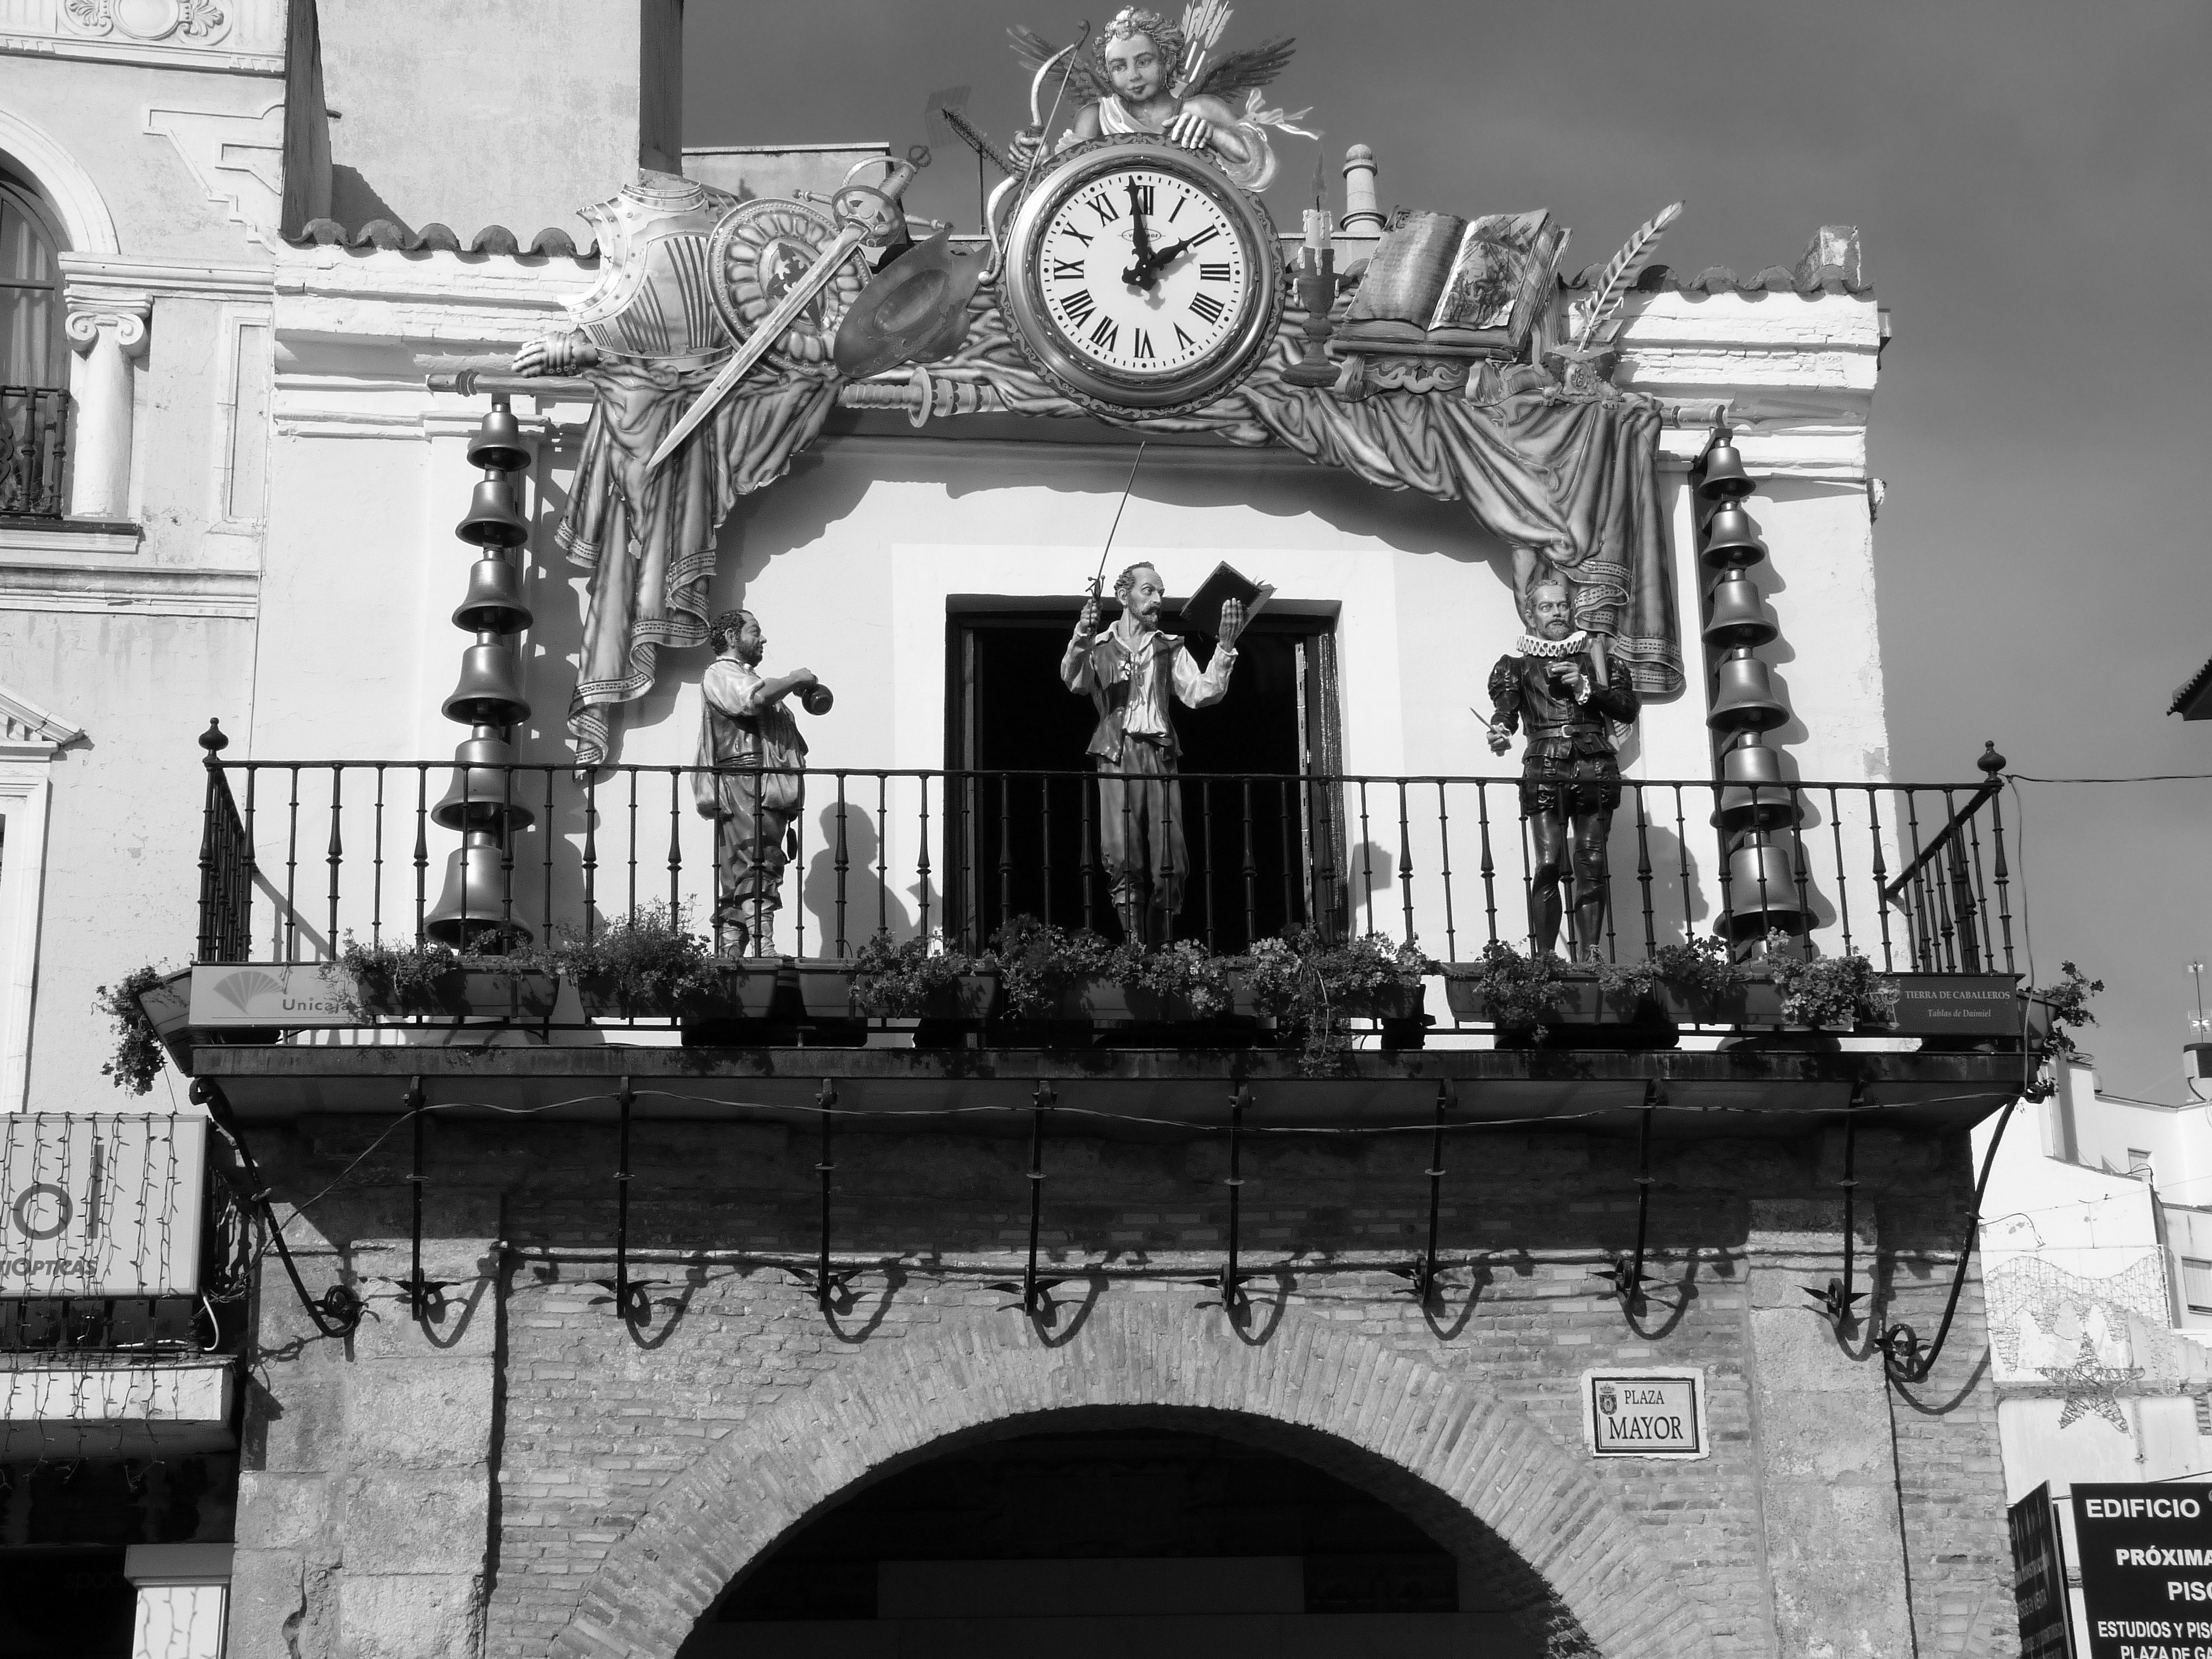
\includegraphics[width=0.8\linewidth]{clockCRbw}
		\caption{Fotografía en blanco y negro}\label{fig:fotoBW}
	\end{subfigure} 
	\caption[Ejemplo de subfiguras]{Ejemplo de inclusión de subfiguras en un mismo entorno (por J. Salido, CC BY-NC-ND)}
	\label{fig:ejSubfigures}
\end{figure}



Mediante el uso de etiquetas (\texttt{\textbackslash label}) es posible incluir referencias cruzadas a subfiguras como la fotografía en blanco y negro de la Fig.~\ref{fig:fotoBW}.

En los trabajos académicos la inclusión de imágenes y figuras que no son propiedad del autor suscitan bastante controversia y son fuente de incumplimiento inadvertido de la ley de propiedad intelectual.\index{plagio!propiedad intelectual} Es importante recordar que \emph{<<el desconocimiento de la ley no exime de su cumplimiento>>} por lo que se recomienda tanto a estudiantes como tutores consultar documentación informativa sobre el uso correcto de figuras en documentos académicos \cite{unican18}. Entre las <<incorrecciones>> más frecuentes al incluir figuras en los documentos académicos se observan:
\begin{itemize}
\item Abuso del derecho de cita. Se produce al incluir, con fines exclusivamente decorativos o ilustrativos de la explicación, una figura sujeta a derechos de uso restringido invocando el derecho de cita (incluso con correcta atribución de la obra).

\item Incorrecta atribución de la obra.\index{atribución} Es habitual confundir al autor de la obra con la fuente de origen de la misma. La fuente es precisa cuando se cita la obra original. Sin embargo, la licencia de muchas obras exige la atribución al autor y la inclusión de la licencia bajo la que se distribuye o hace uso de la misma (véase como ejemplo cómo se realiza una correcta atribución en las Fig.~\ref{fig:ejFigure} y \ref{fig:ejSubfigures} mencionando al autor y la licencia Creative-Commons\footnote{\url{https://creativecommons.org}} bajo la que se rige el uso de la imagen y el mecanismo de título alternativo para que dicha atribución no aparezca en el índice de figuras).\index{Creative Commons}

\item Supresión de denominación de licencia de uso. Al incluir obras de terceros debemos tener presente los términos de distribución de la misma e incluirlos junto a la atribución de su legítimo autor.
\end{itemize}

La inclusión de material de \emph{dominio público}\index{dominio público} o sin restricciones de uso hace innecesaria la atribución al autor pero puede incluirse una nota de agradecimiento.\footnote{Por cortesía de \emph{<x>}.}

\section{Ejemplos de listados}
\label{sec:ejListados}
\index{ejemplos!listados}

Ejemplos más representativos de inclusión de porciones de código 
fuente.\index{listados}

% Ejemplo: Listado Java
% ============
\begin{lstlisting}[language=Java,float=ht,caption={[Código fuente en Java]Ejemplo de código fuente en lenguaje Java},label=lst:java]
// @author www.javadb.com
public class Main {    
// Este método convierte un String a un vector de bytes

public void convertStringToByteArray() {

String stringToConvert = "This String is 15";      
	byte[] theByteArray = stringToConvert.getBytes();        
	System.out.println(theByteArray.length);        
}

public static void main(String[] args) {
	new Main().convertStringToByteArray();
}
}
\end{lstlisting}



\noindent Otro ejemplo.

\begin{lstlisting}[style=C-ruled,float=ht,caption={Ejemplo de código C},label=lst:codC]
// Este código se ha incluido tal cual está en el fichero \LaTeX{}
#include <stdio.h>

int main(int argc, char* argv[]) {
	puts("¡Hola mundo!");
}
\end{lstlisting}


\noindent Ejemplo de entrada por consola.

\begin{lstlisting}[style=consola, numbers=none]
$ gcc -o Hola HolaMundo.c
\end{lstlisting}


\noindent Un ejemplo más. Este en Matlab:
% NOTA: En español soluciona problema con signo % en listados de código Matlab. 
% Si efecto en el resto de idiomas.
\spanishplainpercent
\begin{lstlisting}[style=Matlab-color,float=ht,caption={Ejemplo escrito en Matlab},label=lst:matlab]
function f = fibonacci(n)
 % FIBONACCI  Fibonacci sequence
 %	f = FIBONACCI(n) generates the first n Fibonacci numbers.
 %	Copyright 2014 Cleve Moler
 %	Copyright 2014 The MathWorks, Inc.
f = zeros(n,1); 
f(1) = 1;
f(2) = 2;
for k = 3:n
f(k) = f(k-1) + f(k-2);
end
\end{lstlisting}
\spanishpercent

\subsection{Algoritmos con el paquete \texttt{algorithm2e}}
Como ya se ha comentado en los textos científicos relacionados con las 
TIC\footnote{Por supuesto en un TFG (Trabajo Fin de Grado)\index{TFG} o tesis 
de un centro superior de informática.} (Tecnologías de la Información y 
Comunicaciones) suelen aparecer porciones de código en los que se explica 
alguna función o característica relevante del trabajo que se expone. Muchas 
veces lo que se quiere ilustrar es un algoritmo o método en que se ha 
resuelto un problema abstrayéndose del lenguaje de programación concreto en 
que se realiza la implementación. El paquete 
\texttt{algorithm2e}\footnote{\url{https://osl.ugr.es/CTAN/macros/latex/contrib/algorithm2e/doc/algorithm2e.pdf}}\index{CTAN}
 proporciona un entorno \texttt{algorithm} para la impresión apropiada de 
algoritmos tratándolos como objetos flotantes y con mucha flexibilidad de 
personalización. En el algoritmo \ref{alg:como} se muestra cómo puede 
emplearse dicho paquete. En este curso no se explican las posibilidades del 
paquete más en profundidad, ya que excede el propósito del curso. A todos los 
interesados se les remite a la documentación del mismo.


% Ejemplo:
% ============
\IncMargin{1em}
\begin{algorithm}
\SetKwInOut{Input}{Datos}\SetKwInOut{Output}{Resultado}
\LinesNumbered
\SetAlgoLined

\Input{este texto} 
%\KwIn{este texto}
\Output{como escribir algoritmos con \LaTeX2e}
%\KwOut{como escribir algoritmos con \LaTeX2e}

inicialización\;
\While{no es el fin del documento}{
	leer actual\;
	\eIf{comprendido}{
		ir a la siguiente sección\;
		la sección actual es esta\;
	}{
		ir al principio de la sección actual\;
	}
}

% Aunque el captión aparece abajo siempre se pone arriba como en tablas y listados
\caption{Cómo escribir algoritmos}\label{alg:como}
\end{algorithm}\DecMargin{1em}



\section{Menús, paths y teclas con el paquete \texttt{menukeys}}
Cada vez es más usual que los trabajos en ingeniería exijan el uso de 
software. Para poder especificar de modo elegante el uso menús, pulsación de 
teclas y directorios se recomienda el uso del paquete 
\texttt{menukeys}.\footnote{\url{https://osl.ugr.es/CTAN/macros/latex/contrib/menukeys/menukeys.pdf}}
 \index{CTAN} Este paquete nos permite especificar el acceso a un menú, por 
ejemplo:

\menu{Herramientas:Órdenes:PDFLaTeX}\\

\noindent También un conjunto de teclas. Por ejemplo:
\keys{\ctrl + \shift + T}\\

\noindent O un directorio:
\directory{C:/user/LaTeX/Ejemplos}\\

\noindent Aunque este paquete permite muchas opciones de configuración de los estilos aplicados, no es necesario hacerlo para obtener unos resultados muy elegantes.



\section{Ejemplos de fórmulas matemáticas}
Para que \LaTeX{} pueda incluir muchos símbolos matemáticos es preciso incluir algunos paquetes que ayudan en dicha tarea: \texttt{amsmath}, \texttt{amsfonts}, \texttt{amssymb}. También hay que tener en cuenta que si el tipo principal empleado en el texto es Times y se desea utilizar un tipo coherente en las fórmulas es conveniente emplear el paquete \emph{mathptmx} en vez de \emph{Times}. Pero en este caso es recomendable incluir siempre paquetes adicionales para suministrar las otras dos familias de fuentes escalables (p.~ej.\ \texttt{helvet} para familia \textsf{palo seco} y \texttt{couriers} para \texttt{monoespaciada}). Si no se hace esta última inclusión pueden obtenerse errores de difícil diagnóstico.



\subsection{Fórmulas creadas en línea y con entorno \texttt{equation}}
Es muy sencillo incluir fórmulas matemáticas sencillas en el mismo texto en el que se escribe. Por ejemplo, $c^{2}=a^{2}+b^{2}$ que podría ser la ecuación representativa del teorema de Pitágoras.

Las fórmulas también se pueden separar del texto para que aparezcan destacadas, así:

% Ejemplo: Ecuación no numerada
% ============
\[
c^2  = \int {\left( {a^2  + b^2} \right)}  \cdot dx
\]


Pero si se desea, las ecuaciones pueden ser numeradas de forma automática e incluso utilizar referencias cruzadas a ellas:

% Ejemplo: Ec. numerada.
% ============
% MathType!MTEF!2!1!+-
% feqaeaartrvr0aaatCvAUfeBSjuyZL2yd9gzLbvyNv2CaerbuLwBLn
% hiov2DGi1BTfMBaeXatLxBI9gBaebbnrfifHhDYfgasaacH8srps0l
% bbf9q8WrFfeuY-Hhbbf9v8qqaqFr0xc9pk0xbba9q8WqFfea0-yr0R
% Yxir-Jbba9q8aq0-yq-He9q8qqQ8frFve9Fve9Ff0dmeaabaqaciGa
% caGaaeqabaaaamaaaOqaaiaadogadaahaaWcbeqaaiaaikdaaaGccq
% GH9aqpcaWGHbWaaWbaaSqabeaacaaIYaaaaOGaey4kaSIaamOyamaa
% CaaaleqabaGaaGOmaaaaaaa!3910!
\begin{equation} \label{eq:pitagoras}
	a^{2}=b^{2} + c^{2}
\end{equation}

No hay que preocuparse demasiado por la tipografía empleada en las fórmulas pues \LaTeX{} hace por nosotros <<casi>> todo el trabajo.\footnote{Los matemáticos son muy exquisitos y no se conforman con cualquier cosa, pero nosotros debemos ser mucho menos pretenciosos si queremos resultados rápidos.}

Los ejemplos que aquí se muestran son muy sencillos pero \LaTeX{} proporciona entornos específicos más potentes. Para mostrar algo <<más sofisticado>> añado dos ejemplos más. La ec.~\ref{eq:integral} que es un poquito más compleja y la ec.~\ref{eq:cuadro} que está recuadrada.

% Ejemplo:
% ============
\begin{equation}\label{eq:integral}
	I = \! \int_{-\infty}^\infty f(x)\,dx
\end{equation}

Un ejemplo de alineación de ecuación mediante entorno \texttt{flalign}:\footnote{Otra forma de conseguir el alineamiento a la izquierda de las ecuaciones se consigue añadiendo \texttt{fleqn} como opción de la clase del documento.}
\begin{flalign}
    &f(x) = -1.25x^{2} + 1.5x&
\end{flalign}

En este caso la versión con estrella (\texttt{flalign*}) suprime la numeración de la ecuación.

% Ejemplo: Ec. con recuadro (numeración exterior).
% ============
{\fboxsep 8pt \fboxrule 0.5pt 
%\fboxsep ajusta la separación entre la caja y el elemento recuadrado
%\fboxrule ajusta el espesor de la línea del recuadro
\begin{equation}\label{eq:cuadro}
\fbox{$\displaystyle 
R = \frac{L}{2} \cdot \frac{{\left( {v_d  + v_i } \right)}}{{\left( {v_d  - v_i } \right)}}
$}
\end{equation}
}


Algunos otros cuadros en ecuaciones son p.~ej.\ $x + y = \fbox{$\Omega$}$ o incluso el que se muestra a continuación (ec.~\ref{eq:cuadrogrande}) y que abarca todo el ancho de la línea:\footnote{Adaptado del manual \emph{Documentation for fancybox.sty:
Box tips and tricks for \LaTeX{}} de Timothy Van Zandt (2010).}

% Ejemplo: Ec. con recuadro (numeración interior).
% ============
\newlength{\milong}
\[
	\setlength{\fboxsep}{15pt}
	\setlength{\milong}{\linewidth}
	\addtolength{\milong}{-2\fboxsep}
	\addtolength{\milong}{-2\fboxrule}
	\fbox{%
		\parbox{\milong}{
		\setlength{\abovedisplayskip}{0pt}
		\setlength{\belowdisplayskip}{0pt}
		\begin{equation}\label{eq:cuadrogrande}
		\sqrt[n]{1+x+x^2+x^3+\ldots}
		\end{equation}}}
\]



\subsection{Ecuaciones en varias líneas con entornos \texttt{eqnarray} y \texttt{align}}
A continuación se muestra un ejemplo de ecuación muy larga dividida en varias líneas:

% Ejemplo: Ec. en varias líneas con alineación y sin numeración.
% ============
\begin{eqnarray*}
  \lefteqn{\left(1+x\right)^n = } \\
  & & 1 + nx + \frac{n\left(n-1\right)}{2!}x^2 + \\
  & & \frac{n\left(n-1\right)\left(n-2\right)}{3!}x^3 + \\
  & & \frac{n\left(n-1\right)\left(n-2\right)\left(n-3\right)}{4!}x^4 + \\
  & & \ldots
\end{eqnarray*}
% Apreciar el asterisco en la ecuación anterior para evitar que todas las líneas de la ecuación aparezcan numeradas.

También se puede escribir varias ecuaciones en líneas sucesivas alineadas por algún elemento como se hace en el siguiente ejemplo de uso del entorno \texttt{align}:

% Ejemplo: Ecs. en varias líneas con alineación y manejo de la numeración.
% ============
\begin{align}
f(x) & = \cos x \\
f'(x) & = -\sin x \\
\int_{0}^{x} f(y)dy & = \sin x \nonumber
\end{align}

\noindent En este último ejemplo se observa también cómo es posible suprimir la numeración de una de las ecuaciones con el comando (\texttt{\textbackslash nonumber}).

Para terminar, un ejemplo más del control del espaciado horizontal empleando el entorno \texttt{array}:

% Ejemplo:
% ============
\[f(n) = \left\{ 
\begin{array}{l l}
  n/2 & \quad \mbox{si $n$ es par}\\
  -(n+1)/2 & \quad \mbox{si $n$ es impar}\\ \end{array} \right. \]



\chapter{Objetivo}
\label{cap:Objetivo}

Introduce y motiva la problemática (i.e.\emph{\ ¿cuál es el problema que se plantea y por qué es interesante su resolución?})

Debe concretar y exponer detalladamente el problema a resolver, el entorno de 
trabajo, la situación y qué se pretende obtener. También puede contemplar las 
limitaciones y condicionantes a considerar para la resolución del problema 
(lenguaje de construcción, equipo físico, equipo lógico de base o de apoyo, 
etc.). Si se considera necesario, esta sección puede titularse 
\emph{Objetivos del TFG e hipótesis de trabajo}. En este caso, se añadirán 
las hipótesis de trabajo que el alumno pretende demostrar con su TFG.\index{TFG}

Una de las tareas más complicadas al proponer un TFG es plantear su \textsf{Objetivo}. La dificultad deriva de la falta de consenso respecto de lo que se entiende por \emph{objetivo} en un trabajo de esta naturaleza. En primer lugar se debe distinguir entre dos tipos de objetivo:

\begin{enumerate}
	\item La \emph{finalidad específica} del TFG que se plantea para resolver una problemática concreta aplicando los métodos y herramientas adquiridos durante la formación académica. Por ejemplo, \emph{<<Desarrollo de una aplicación software para gestionar reservas hoteleras \emph{on-line}>>}.
	
	\item El \emph{propósito académico} que la realización de un TFG tiene en la formación de un graduado. Por ejemplo, la \emph{adquisición de competencias específicas de la especialización} cursada.
\end{enumerate}

En el ámbito de la memoria del TFG se tiene que definir el primer tipo de objetivo, mientras que el segundo tipo es el que se añade al elaborar la propuesta de un TFG presentada ante un comité para su aprobación. \emph{Este segundo tipo de objetivo no debe incluirse en la memoria y en todo caso solo debe hacerse en la sección de conclusiones finales.}\footnote{En lagunas titulaciones es obligatorio que la memoria explique las competencias específicas alcanzadas con la realización del trabajo.}

Un objetivo bien planteado debe estar determinado en términos del \emph{<<producto final>>} esperado que resuelve un problema específico. Es por tanto un sustantivo que debería ser \emph{concreto} y \emph{medible}. El \textsf{Objetivo} planteado puede pertenecer una de las categorías que se indica a continuación:
\begin{itemize}
	\item \emph{Diseño y desarrollo de <<artefactos>>}\index{artefacto} 
	(habitual en las ingenierías),
	\item \emph{Estudio} que ofrece información novedosa sobre un tema (usual en las ramas de ciencias y humanidades), y
	\item \emph{Validación\index{validación} de una 
	hipótesis}\index{hipótesis} de partida (propio de los trabajos 
	científicos y menos habitual en el caso de los TFG).
\end{itemize}

Estas categorías no son excluyentes, de modo que es posible plantear un trabajo cuyo objetivo sea el diseño y desarrollo de un <<artefacto>> y este implique un estudio previo o la validación de alguna hipótesis para guiar el proceso. En este caso y cuando el objetivo sea lo suficientemente amplio puede ser conveniente su descomposición en elementos más simples hablando de \emph{subobjetivos}. Por ejemplo, un programa informático puede descomponerse en módulos o requerir un estudio previo para plantear un nuevo algoritmo que será preciso validar. La descomposición de un objetivo principal en subobjetivos\index{subobjetivo} 
u objetivos secundarios debería ser natural (no forzada), bien justificada y 
sólo pertinente en los trabajos de gran amplitud.

Junto con la definición del objetivo del trabajo se puede especificar los \emph{requisitos} que debe satisfacer la solución aportada. Estos requisitos especifican \emph{características} que debe poseer la solución y \emph{restricciones} que acotan su alcance. En el caso de un trabajo cuyo objetivo es el desarrollo de un <<artefacto>> los requisitos pueden ser \emph{funcionales} y \emph{no funcionales}.

Al redactar el objetivo de un TFG se debe evitar confundir los medios con el 
fin. Así es habitual encontrarse con objetivos definidos en términos de las 
\emph{acciones} (verbos) o \emph{tareas}\index{tarea} que será preciso 
realizar para llegar al verdadero objetivo. Sin embargo, a la hora de 
planificar el desarrollo del trabajo si es apropiado descomponer todo el 
trabajo en \emph{hitos} y estos en \emph{tareas} para facilitar dicha 
\emph{planificación}.

La categoría del objetivo planteado justifica modificaciones en la organización genérica de la memoria del trabajo. Así en el caso de estudios y validación de hipótesis el apartado de resultados y conclusiones debería incluir los resultados de experimentación y los comentarios de cómo dichos resultados validan o refutan la hipótesis planteada.


\chapter{Metodología}
\label{cap:Metodologia}

En este capítulo se debe detallar las metodologías\index{metodología} 
empleadas para planificación y desarrollo del trabajo, así como explicar de 
modo claro y conciso cómo se han aplicado dichas metodologías.

A continuación se incluye una guía rápida que puede ser de gran utilidad en la elaboración de este capítulo.

\section{Guía rápida de las metodologías de desarrollo de software}

\subsection{Proceso de desarrollo de software}

El \textbf{proceso de desarrollo de software} se denomina también 
\textbf{ciclo de vida del desarrollo del software} (\emph{SDLC, Software 
Development Life-Cycle})\index{SDLC}\index{Life-Cycle} y cubre las siguientes 
actividades:

\begin{enumerate}
\item \textbf{Obtención y análisis de requisitos}\index{requisitos} 
(\emph{requirements analysis}). Es la definición de la funcionalidad del 
software a desarrollar. Suele requerir entrevistas entre los ing. de software 
y el cliente para obtener el `qué' y `cómo'. Permite obtener una 
\emph{especificación funcional} del software.

\item \textbf{Diseño} (\emph{SW design}).\index{diseño} Consiste en la 
definición de la arquitectura, los componentes, las interfaces y otras 
características del sistema o sus componentes.

\item \textbf{Implementación} (\emph{SW construction and coding}). Es el
  proceso de codificación del software en un lenguaje de programación.
  Constituye la fase en que tiene lugar el desarrollo de software.

\item \textbf{Pruebas} (\emph{testing and verification}).\index{testing} 
Verificación del correcto funcionamiento del software para detectar fallos lo 
antes posible. Persigue la obtención de software de calidad. Consisten en 
pruebas de \emph{caja negra} y \emph{caja blanca}. Las primeras comprueban 
que la funcionalidad es la esperada y para ello se verifica que ante un 
conjunto amplio de entradas, la salida es correcta. Con las segundas se 
comprueba la robustez del código sometiéndolo a pruebas cuya finalidad es 
provocar fallos de software. Esta fase también incorpora la \emph{pruebas de 
integración} en las que se verifica la interoperabilidad del sistema con 
otros existentes.

\item \textbf{Documentación} (\emph{documentation}). Persigue facilitar la mejora continua del software y su mantenimiento.

\item \textbf{Despliegue} (\emph{deployment}).\index{despliegue} Consiste en 
la instalación del software en un entorno de producción y puesta en marcha 
para explotación. En ocasiones implica una fase de \emph{entrenamiento} de 
los usuarios del software.

\item \textbf{Mantenimiento} (\emph{maintenance}).\index{mantenimiento} Su 
propósito es la resolución de problemas, mejora y adaptación del software en 
explotación.
\end{enumerate}




\subsection{Metodologías de desarrollo software}
\emph{Las metodologías son el modo en que las fases del proceso software se organizan e interaccionan para conseguir que dicho proceso sea reproducible y predecible para aumentar la productividad y la calidad del software.}

Una metodología es una colección de:

\begin{itemize}
\item \textbf{Procedimientos} (indican cómo hacer cada tarea y en qué momento),
\item \textbf{Herramientas} (ayudas para la realización de cada tarea), y
\item \textbf{Ayudas documentales}.
\end{itemize}

Cada metodología es apropiada para un tipo de proyecto dependiendo de sus 
características técnicas, organizativas y del equipo de trabajo. En los 
entornos empresariales es obligado, a veces, el uso de una metodología 
concreta (p.~ej. para participar en concursos públicos). El estándar 
internacional ISO/IEC 12270\index{ISO/IEC 12270} describe el método para 
seleccionar, implementar y monitorear el ciclo de vida del software.

Mientras que unas intentan sistematizar y formalizar las tareas de diseño, otras aplican técnicas de gestión de proyectos para dicha tarea. Las metodologías de desarrollo se pueden agrupar dentro de varios enfoques según se señala a continuación.

\begin{enumerate}
\item \textbf{Metodología de Análisis y Diseño de Sistemas Estructurados} 
(\emph{SSADM, Structured Systems Analysis and Design 
Methodology}).\index{SSADM} Es uno de los paradigmas más antiguos. En esta 
metodología se emplea un modelo de desarrollo en cascada 
(\emph{waterfall}).\index{modelo!waterfall@\emph{waterfall}} Las fases de 
desarrollo tienen lugar de modo secuencial. Una fase comienza cuando termina 
la anterior. Es un método clásico poco flexible y adaptable a cambios en los 
requisitos. Hace especial hincapié en la planificación derivada de una 
exhaustiva definición y análisis de los requisitos. Son metodologías que no 
lidian bien con la flexibilidad requerida en los proyectos de desarrollo 
software. Derivan de los procesos en  ingeniería tradicionales y están 
enfocadas a la reducción del riesgo. Emplea tres técnicas clave:

\begin{itemize}
\item Modelado lógico de datos (\emph{Logical Data 
Modelling}),\index{modelado}
\item Modelado de flujo de datos (\emph{Data Flow Modelling}), y
\item Modelado de Entidades y Eventos (\emph{Entity Event
  Modelling}).
\end{itemize} 

\item \textbf{Metodología de Diseño Orientado a Objetos} (\emph{OOD,  
Object-Oriented Design}).\index{OOD} Está muy ligado a la \index{OOP}OOP (Programación 
Orientada a Objetos) en que se persigue la reutilización. A diferencia del 
anterior, en este paradigma los datos y los procesos se combinan en una única 
entidad denominada \emph{objetos} (o clases). Esta orientación pretende que 
los sistemas sean más modulares para mejorar la eficiencia, calidad del 
análisis y el diseño. Emplea extensivamente el Lenguaje Unificado de Modelado 
(UML)\index{UML} para especificar, visualizar, construir y documentar los 
artefactos de los sistemas software y  también el modelo de negocio. UML 
proporciona una serie diagramas de básicos para modelar un sistema: 

\begin{itemize}
\item Diagrama de Clase (\emph{Class Diagram}). Muestra los objetos del sistema y sus relaciones. 
\item Diagrama de Caso de Uso (\emph{Use Case Diagram}). Plasma la
  funcionalidad del sistema y quién interacciona con él.
\item Diagrama de secuencia (\emph{Sequence Diagram}). Muestra los eventos que se
  producen en el sistema y como este reacciona ante ellos. 
\item Modelo de Datos (\emph{Data Model}).
\end{itemize} 
                               
\item \textbf{Desarrollo Rápido de Aplicaciones} (\emph{RAD, Rapid 
Application Developmnent}).\index{RAD} Su filosofía es sacrificar calidad a 
cambio de poner en producción el sistema rápidamente con la funcionalidad 
esencial. Los procesos de especificación, diseño e implementación son 
simultáneos. No se realiza una especificación detallada y se reduce la 
documentación de diseño. El sistema se diseña en una serie de pasos, los 
usuarios evalúan cada etapa en la que proponen cambios y nuevas mejoras. Las 
interfaces de usuario se desarrollan habitualmente mediante sistemas 
interactivos de desarrollo. En vez de seguir un modelo de desarrollo en 
cascada sigue un modelo en espiral (Boehm).\index{modelo!espiral} La clave de 
este modelo es el desarrollo continuo que ayuda a minimizar los riesgos. Los 
desarrolladores deben definir las características de mayor prioridad. Este 
tipo de desarrollo se basa en la creación de prototipos y realimentación 
obtenida de los clientes para definir e implementar más características hasta 
alcanzar un sistema aceptable para despliegue.

\item \textbf{Metodologías Ágiles}. \emph{"[...] envuelven un enfoque para la 
toma de decisiones en los proyectos de software, que se refiere a métodos de 
ingeniería del software basados en el desarrollo iterativo e incremental, 
donde los requisitos y soluciones evolucionan con el tiempo según la 
necesidad del proyecto. Así el trabajo es realizado mediante la colaboración 
de equipos auto-organizados y multidisciplinarios, inmersos en un proceso 
compartido de toma de decisiones a corto plazo. Cada iteración del ciclo de 
vida incluye:  planificación, análisis de requisitos, diseño, codificación, 
pruebas y  documentación. Teniendo gran importancia el concepto de 
"Finalizado" (Done), ya que el objetivo de cada iteración no es agregar toda 
la funcionalidad para justificar el lanzamiento del producto al mercado, sino 
incrementar el valor por medio de "software que funciona" (sin errores). Los 
métodos ágiles enfatizan las comunicaciones cara a cara en vez de la 
documentación. [...]"}\footnote{Fuente: Wikipedia}\index{Wikipedia}
\end{enumerate}

\subsection{Proceso de testing}\index{testing}

\begin{enumerate}
\item \emph{Pruebas modulares} (pruebas unitarias). Su propósito es hacer pruebas sobre un módulo tan pronto como sea posible. Las \emph{pruebas unitarias} que comprueban el correcto funcionamiento de una unidad de código. Dicha unidad elemental de código consistiría en cada función o procedimiento, en el caso de programación estructurada y cada clase, para la programación orientada a objetos. Las características de una prueba unitaria de calidad son: \emph{automatizable} (sin intervención manual), \emph{completa},  \emph{reutilizable}, \emph{independiente} y \emph{profesional}.

\item \emph{Pruebas de integración}. Pruebas de varios módulos en conjunto para comprobar su interoperabilidad.

\item \emph{Pruebas de caja negra}.

\item \emph{Beta testing}.

\item \emph{Pruebas de sistema y aceptación}.

\item \emph{Training}.
\end{enumerate}






\subsection{Herramientas CASE (\emph{Computer Aided Software Engineering})}

Las herramientas CASE\index{CASE} están destinadas a facilitar una o varias 
de las tareas implicadas en el ciclo de vida del desarrollo de software. Se 
pueden dividir en la siguientes categorías:

\begin{enumerate}
\item Modelado y análisis de negocio.
\item Desarrollo. Facilitan las fases de diseño y construcción.
\item Verificación y validación.
\item Gestión de configuraciones.
\item Métricas y medidas.
\item Gestión de proyecto. Gestión de planes, asignación de tareas, planificación, etc.
\end{enumerate}




\subsubsection{IDE (Integrated Development Environment)}\index{IDE}
\begin{multicols}{2}
\begin{itemize}
\item \href{https://notepad-plus-plus.org/}{Notepad++}
\item \href{https://code.visualstudio.com/}{Visual Studio Code}
\item \href{https://atom.io/}{Atom}
\item \href{https://www.gnu.org/s/emacs/}{GNU Emacs}
\item \href{https://netbeans.org/}{NetBeans}
\item \href{https://eclipse.org/}{Eclipse}
\item \href{https://www.qt.io/ide/}{Qt Creator}
\item \href{http://www.jedit.org/}{jEdit}
\item \href{https://www.jetbrains.com/idea/}{ItelliJ IDEA}
\end{itemize}
\end{multicols}



\subsubsection{Depuración}\index{depuración}
\begin{itemize}
\item \href{https://www.gnu.org/s/gdb/}{GNU Debugger}
\end{itemize}


\subsubsection{Testing}\index{testing}
\begin{multicols}{2}
\begin{itemize}
\item \href{http://junit.org}{JUnit}. Entorno de pruebas para Java.
\item \href{http://cunit.sourceforge.net/}{CUnit}. Entorno de pruebas para C.
\item \href{https://wiki.python.org/moin/PyUnit}{PyUnit}. Entorno de pruebas para Python.
\end{itemize}
\end{multicols}

\subsubsection{Repositorios y control de versiones}\index{control de 
versiones}
\begin{multicols}{2}
\begin{itemize}
\item \href{https://git-scm.com/}{Git}
\item \href{https://www.mercurial-scm.org/}{Mercurial}
\item \href{https://github.com/}{Github}
\item \href{https://bitbucket.org/}{Bitbucket}
\item \href{https://www.sourcetreeapp.com/}{SourceTree}
\end{itemize}
\end{multicols}


\subsubsection{Documentación}
\begin{multicols}{2}
\begin{itemize}
\item \href{https://www.latex-project.org/}{\LaTeX}
\item \href{https://markdown.es/}{Markdown}
\item \href{http://www.stack.nl/\%7Edimitri/doxygen/index.html}{Doxygen}
\item \href{http://mtmacdonald.github.io/docgen/docs/index.html}{DocGen}
\item \href{http://pandoc.org/}{Pandoc}
\end{itemize}
\end{multicols}



\subsubsection{Gestión y planificación de proyectos}\index{planificación}
\begin{multicols}{2}
\begin{itemize}
\item \href{https://trello.com/}{Trello}
\item \href{https://es.atlassian.com/software/jira}{Jira}
\item \href{https://asana.com/}{Asana}
\item \href{https://slack.com/}{Slack}
\item \href{https://basecamp.com/}{Basecamp}
\item \href{https://www.teamwork.com/project-management-software}{Teamwork Projects}
\item \href{https://www.zoho.com/projects/}{Zoho Projects}
\end{itemize}
\end{multicols}


\subsection{Fuentes de información adicional}
\begin{itemize}
\item \href{https://leankit.com/blog/2019/03/top-6-software-development-methodologies/}{Top
  6 Software Development Methodologies}. Maja Majewski. Planview
  LeanKit, 2019.
\item \href{https://acodez.in/12-best-software-development-methodologies-pros-cons/}{12
  Best software development methodologies with pros and cons}. acodez,
  2018.
\item \href{http://www.itinfo.am/eng/software-development-methodologies/}{Software
  Development Methodologies}. Association of Modern Technologies
  Professionals, 2019.
\end{itemize}

\chapter{Resultados}
\label{cap:Resultados}

En esta sección se describirá la aplicación del método de trabajo presentado en el capítulo \ref{cap:Metodologia},  mostrando los elementos (modelos, diagramas, especificaciones, etc.) más importantes. 

Este apartado debe explicar cómo el empleo de la metodología permite satisfacer tanto el objetivo principal como los específicos planteados en el TFG así como los requisitos exigidos (según exposición en cap.~\ref{cap:Objetivo}).
\chapter{Conclusiones}
\label{cap:Conclusiones}

En este capítulo se realizará un juicio crítico y discusión sobre los resultados obtenidos. \emph{Cuidado, esta discusión no debe confundirse con una valoración del enriquecimiento personal que supone la realización del trabajo como culminación de una etapa académica}. Aunque de gran importancia, esta última valoración debe quedar fuera de la memoria del trabajo y solo debe ahondarse en ella ante requerimiento explícito del comité en el acto de defensa.

Si es pertinente deberá incluir información sobre trabajos derivados como publicaciones o ponencias en preparación, así como trabajos futuros \emph{(solo si estos están iniciados o planificados en el momento que se redacta el texto)}. Evitar hacer una lista de posibles mejoras. Contrariamente a lo que alguno pueda pensar generalmente aportan impresión de trabajo incompleto o inacabado.\footnote{Puede reflexionarse en ello por si en la defensa del trabajo se pregunta sobre estas posibles mejoras.}


\section{Justificación de competencias adquiridas}
Es muy importante recordar que según la normativa vigente, el capítulo de conclusiones debe incluir \emph{obligatoriamente} un apartado destinado a justificar la aplicación en el TFG de competencias específicas (dos o más) asociadas a la tecnología específica cursada.\index{competencias@\textbf{competencias}}

En el TFG se han trabajado las competencias correspondientes a la Tecnología Específica de \emph{[poner lo que corresponda]}:

\begin{description}
\item[Código de la competencia 1:] \emph{[Texto de la competencia 1]}. Explicación de cómo dicha competencia se ha trabajado en el TFG.
\item[Código de la competencia 2:] \emph{[Texto de la competencia 2]}. Explicación de cómo dicha competencia se ha trabajado en el TFG.
\end{description}

\dots otras más si las hubiera.


\section{Planificación y costes}
En este capítulo se puede incluir una valoración del trabajo realizado en el que se justifique el tiempo dedicado al TFG teniendo en cuenta que este tiene asignados 12 créditos ECTS\index{ECTS} que se traducen en {300-360} horas totales. En este sentido una correcta planificación del TFG debería garantizar que el trabajo se realice dentro de la horquilla señalada. Queda a criterio del tribunal la evaluación de valores extremos por defecto o exceso en función de los resultados obtenidos.

Es muy importante que todas las justificaciones aportadas se sustenten no solo en juicios de valor sino en evidencias tangibles como: historiales de actividad, repositorios de código y documentación, porciones de código, trazas de ejecución, capturas de pantalla, demos, etc.




% -------------------------


%--- BACKMATTER
%\backmatter (se comenta para que los apéndices puedan aparecer después de la bibliografía)


% -------------------------
%
%--- BIBLIOGRAFÍA
%
% -------------------------
% BEGIN_FOLD
% OJO: Todas las referencias deben estar citadas en el texto)
% EDITAR: Comentar línea siguiente
\nocite{*} % INCLUIDO para ver cómo queda, pero comentar en versión final.

\cleardoublepage % OJO: Necesario para ajustar el avance de página
\phantomsection  % OJO: Ojo necesario con hyperref.
\addcontentsline{toc}{chapter}{\bibname} % Añade la bibliografía al Índice de contenidos. Se debe mantaner cuando se desean subbibliografías.
%---
% Opción 1: Bibliografía con todas las fuentes en un apartado.
%---
\printbibliography
%---

%---
% Opción 2: Bibliografía con secciones separadas.
%---
%\printbibheading
% Se puede incluir un apartado de fuentes de consulta no citadas
% Como no están citadas es preciso incluir comando \nocite{<key>}
% Se añaden palabras clave a las entradas en el fichero *.bib para poder diferenciarlas
%\printbibliography[heading=subbibliography,keyword=consulta,title={Fuentes de consulta}]
%\printbibliography[heading=subbibliography,keyword=url,title={Direcciones de Internet}]
% -------------------------
% END_FOLD



% -------------------------
%
%--- ANEXOS: Comentar si no se desean incluir. [OPT.]
% Mover si se desea que aparezcan antes de la bobliografía.
%
% -------------------------
%BEGIN_FOLD
\appendix
\portadaAnexos % OPT. Añade una portada para anexos

% Tras este punto los capítulos se numeran con letras.
% Aquí todos los apéndices necesarios
\chapter{El primer anexo}
\label{cap:AnexoA}

Los anexos se incluirá de modo opcional material suplementario que podrá consistir en breves manuales, listados de código fuente, esquemas, planos, etc. Se recomienda que no sean excesivamente voluminosos, aunque su extensión no estará sometida a regulación por afectar esta únicamente al texto principal. 

\paragraph{Bibliografía}\index{bibliografía}
Esta sección, que si se prefiere puede titularse 
«Referencias»,\index{referencias} incluirá un listado por orden alfabético 
(primer apellido del primer autor) con todas las obras en que se ha basado 
para la realización del TFG\index{TFG} en las que se especificará: autor/es, 
título, editorial y año de publicación. Solo se incluirán en esta sección las 
referencias bibliográficas que hayan sido citadas en el documento. Todas las 
fuentes consultadas no citadas en el documento deberían incluirse en una 
sección opcional denominada <<Material de consulta>>, aunque preferiblemente 
estas deberían incluirse como referencias en notas a pie de página a lo largo 
del documento.

Se usará método de citación numérico con el número de la referencia empleada entre corchetes. La cita podrá incluir el número de página concreto de la referencia que desea citarse. Debe tenerse en cuenta que el uso correcto de la citación implica que debe quedar claro para el lector cuál es el texto, material o idea citado. Las obras referenciadas sin mención explícita o implícita al material concreto citado deberían considerarse material de consulta y por tanto ser agrupados como «Material de consulta» distinguiéndolas claramente de aquellas otras en las que si se recurre a la citación.

Cuando se desee incluir referencias a páginas genéricas de la Web sin mención expresa a un artículo con título y autor definido, dichas referencias podrán hacerse como notas al pie de página o como un apartado dedicado a las «Direcciones de Internet».

Todo el material ajeno deberá ser citado convenientemente sin contravenir los términos de las licencias de uso y distribución de dicho material. Esto se extiende al uso de diagramas y fotografías. El incumplimiento de la legislación vigente en materia de protección de la propiedad intelectual es responsabilidad exclusiva del autor independientemente de la cesión de derechos que este haya convenido.

%De este modo será responsable legal ante cualquier acción judicial derivada del incumplimiento de los preceptos aplicables. Así mismo ante dicha circunstancia los órganos académicos se reservan el derecho a imponer al autor la sanción administrativa que se estime pertinente. 

\paragraph{Índice Temático}\index{Indice Temático@Índice Temático}
Este índice es opcional y se empleará como índice para encontrar los temas tratados en el trabajo. Se organizará de modo alfabético indicando el número de página(s) en el que se aborda el tema concreto señalado.
 % Apéndice A (opcionales)

%---








% -------------------------
%
% OPT.: ÍNDICE TEMÁTICO: Comentar si no se desean incluir.
%
% -------------------------
% CONSEJO: Incluir los comandos mientras se escribe cada capítulo ya que hacerlo al final resulta tedioso.
\cleardoublepage % OJO: Necesario para ajustar el avance de página
\phantomsection  % OJO: Ojo necesario con hyperref.
% EDITAR: Si se desea cambiar el nombre del índice temático
%\renewcommand{\indexname}{Título del índice}
\addcontentsline{toc}{chapter}{\indexname} % Añade al Índice de contenidos.
\printindex  % Facilitado por makeidx (opcional, si no se usa no se imprime)
%---
%END_FOLD
\end{document}